
% Template file for ACCV 2009
%\documentclass[runningheads]{llncs}
%In order to omit page numbers and running heads
%please use the following line instead of the first command line:
\documentclass{acmsiggraph}                     % final
%Furthermore change the line \pagestyle{headings} to
%\pagestyle{empty}
\usepackage[scaled=.92]{helvet}

\usepackage{times}

\usepackage{graphicx}
\usepackage{amsmath}

%% The 'graphicx' package allows for the inclusion of EPS figures.

%% use this for zero \parindent and non-zero \parskip, intelligently.

\usepackage{parskip}

%% Optional: the 'caption' package provides a nicer-looking replacement
%% for the standard caption environment. With 'labelfont=bf,'textfont=it',
%% caption labels are bold and caption text is italic.

\usepackage[labelfont=bf,textfont=it]{caption}
\usepackage{subfig}

%% If you are submitting a paper to the annual conference, please replace
%% the value ``0'' below with the numeric value of your OnlineID.
%% If you are not submitting this paper to the annual conference,
%% you may safely leave it at ``0'' -- it will not be included in the output.

\onlineid{0}

%% Paper title.

\title{Lightweight 3D Modeling of Urban Buildings From Range Data}
\author{Weihong Li\thanks{e-mail: wli@gc.cuny.edu}\\ City College of New York / CUNY %
\and George Wolberg\thanks{e-mail: wolberg@cs.ccny.cuny.edu}\\ City College of New York / CUNY %
\and Siavash Zokai\thanks{e-mail: zokai@brainstormllc.com}\\ Brainstorm Technology LLC}

%% Keywords that describe your work.

\keywords{3D modeling, urban buildings, range data, point clouds, geometry compression}

\newcommand{\Eq}[1] {Eq.~(\ref{eq:#1})}
\newcommand{\Fig}[1]{Fig.~\ref{fig:#1}}
\newcommand{\Sec}[1]{Sec.~\ref{sec:#1}}
\newcommand{\Eqs}   {Eqs.~}
\newcommand{\Figs}  {Figs.~}
\newcommand{\Tbl}[1]{Table~\ref{tbl:#1}}
\newcommand{\Etal}  {{\it et al.}}
\newcommand{\Figa}[1]{Fig.~\ref{fig:#1}(a)}
\newcommand{\Figb}[1]{Fig.~\ref{fig:#1}(b)}
\newcommand{\Figc}[1]{Fig.~\ref{fig:#1}(c)}
\newcommand{\Figd}[1]{Fig.~\ref{fig:#1}(d)}

\graphicspath{{figures/}}

%%%%%% START OF THE PAPER %%%%%%

\begin{document}

\teaser{
\begin{center}
\begin{tabular}{cccc}
%	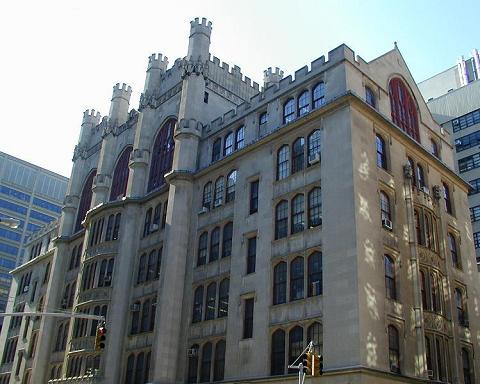
\includegraphics[width=1.5in]{HunterPhoto.jpg} &
	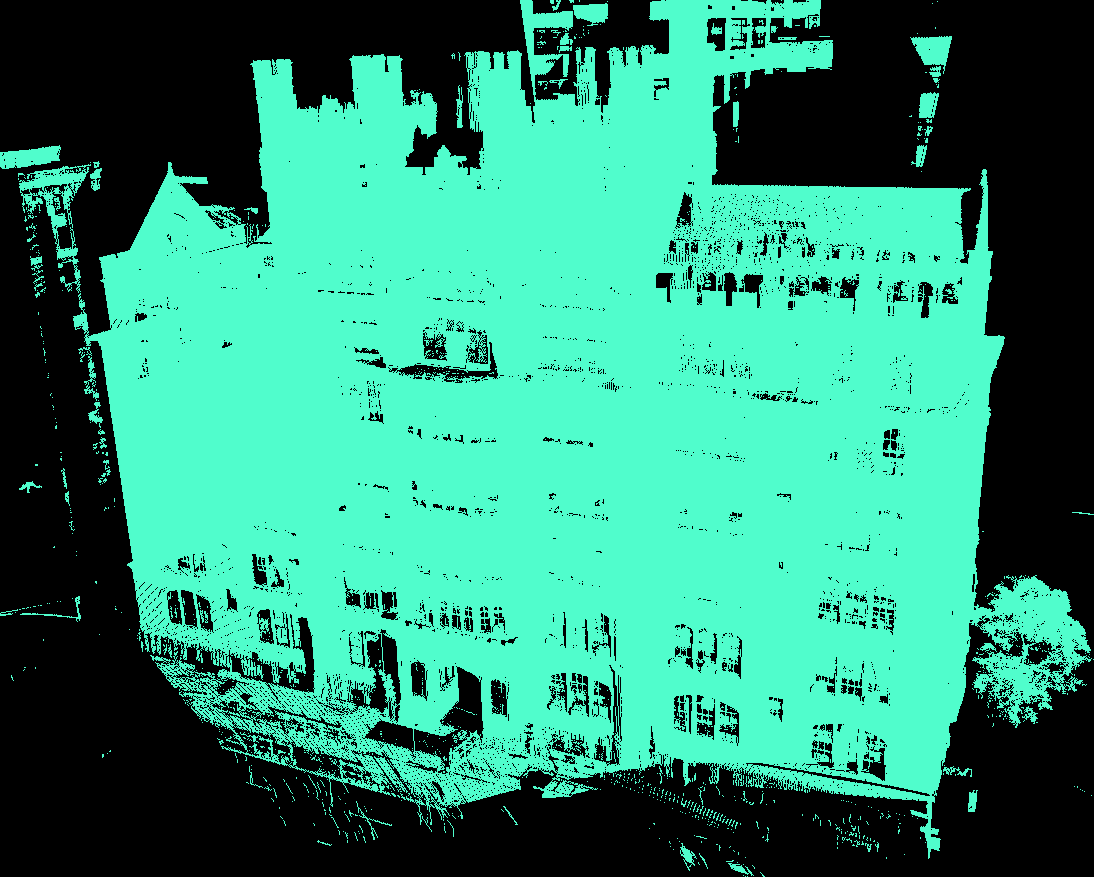
\includegraphics[width=1.5in]{point_cloud.png} &
	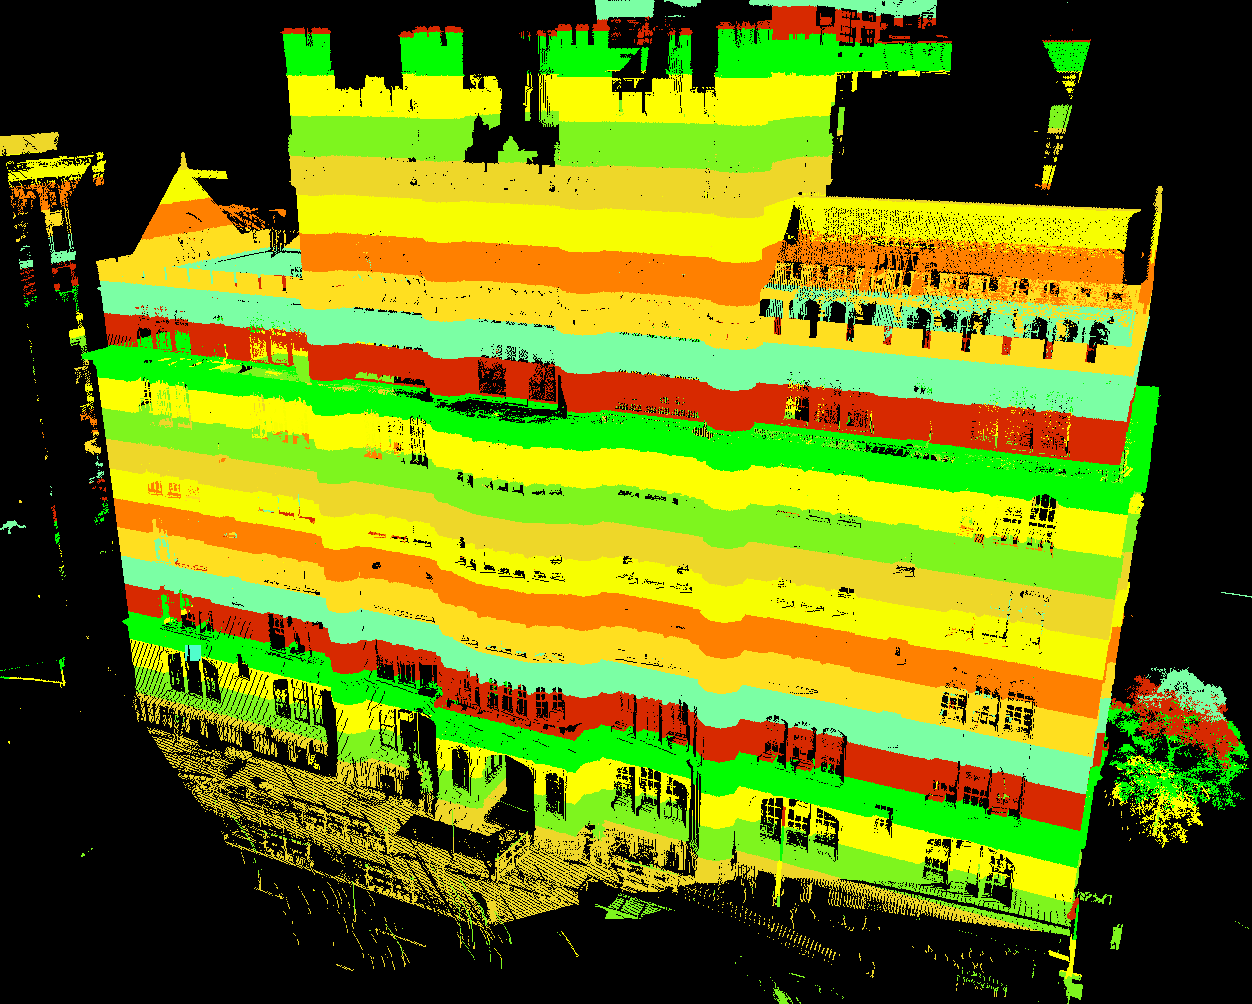
\includegraphics[width=1.5in]{slab_noplanar.png} &
	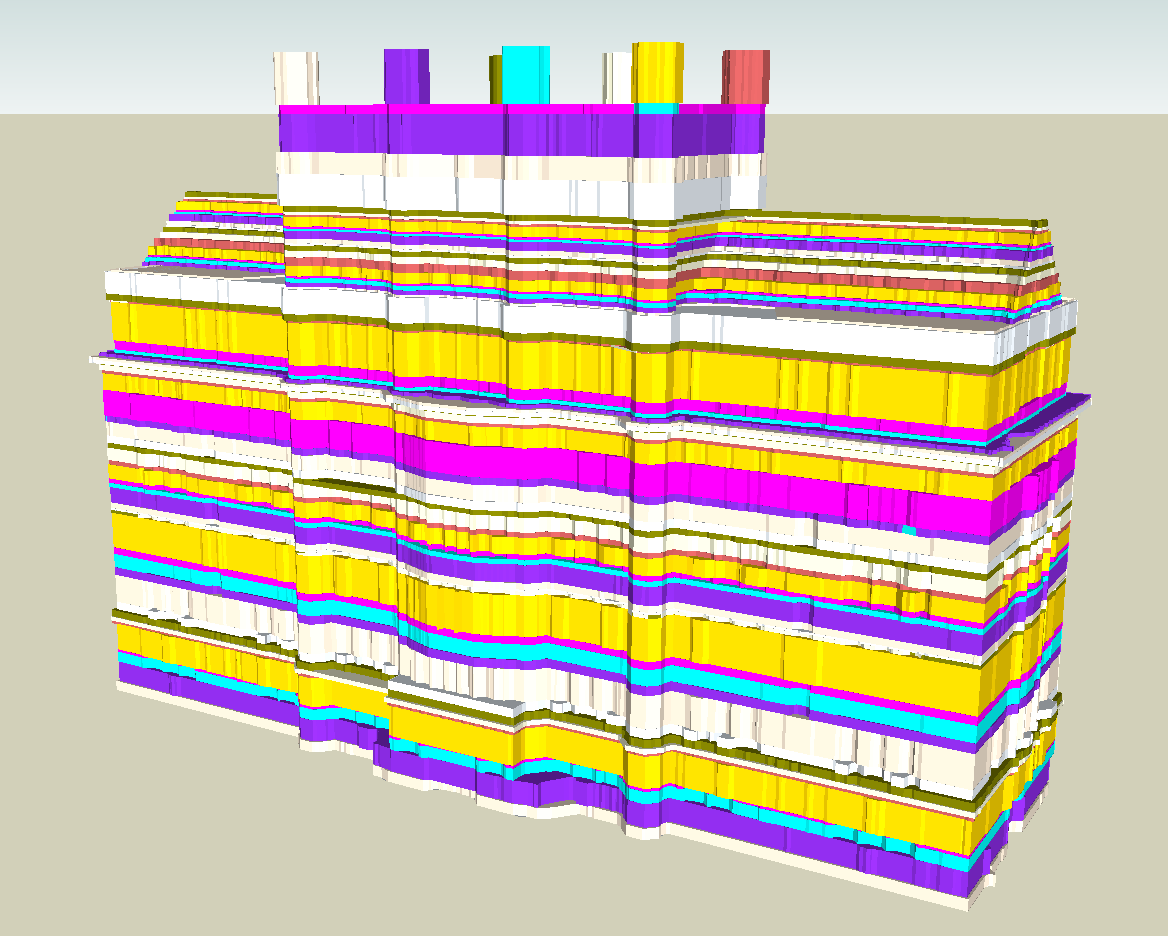
\includegraphics[width=1.5in]{IR_skp_color_face_1000_8_4_paper.png} &
	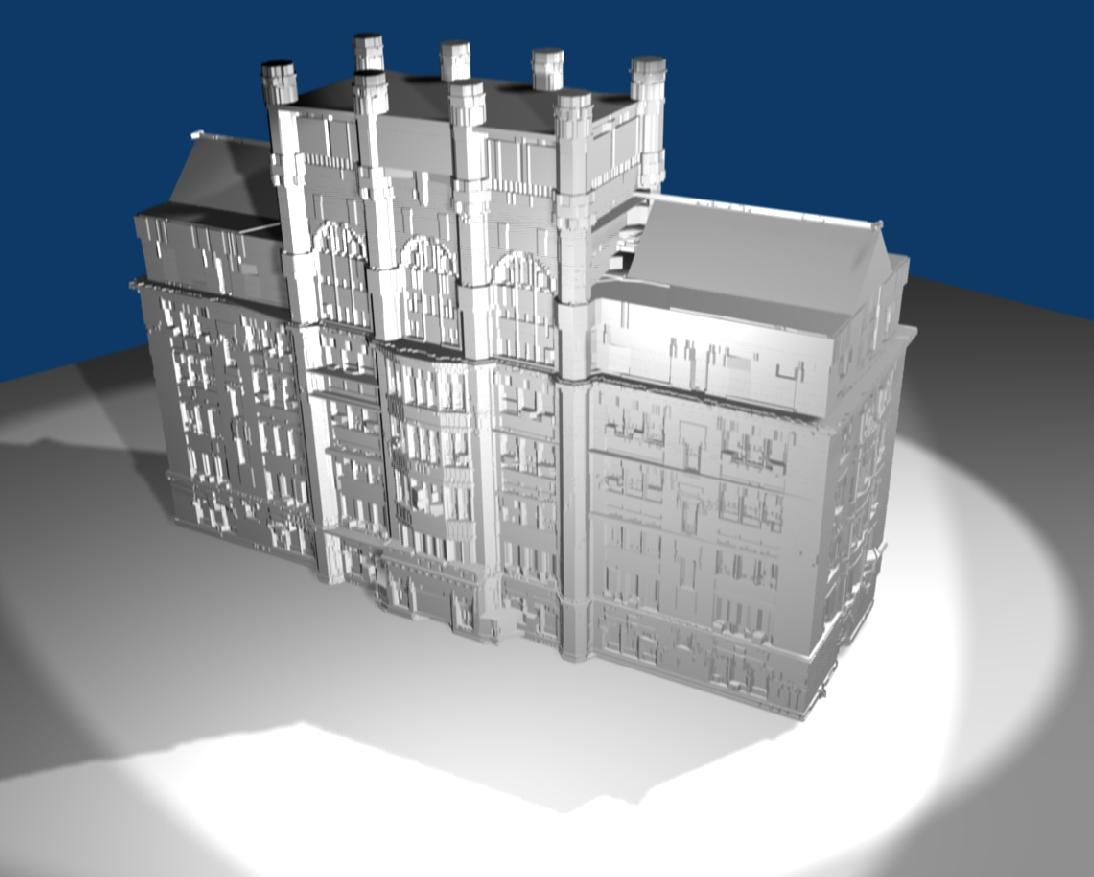
\includegraphics[width=1.5in]{HunterShaded.jpg} \\
	(a) & (b) & (c) & (d) \\
\end{tabular}
\end{center}
\caption{
%(a) A snapshot of the 3D point cloud assembled by registering multiple scans.
(a) A picture of the building to be modeled.
(b) A snapshot of the 3D point cloud assembled by registering multiple scans.
(c) The slabs of the 3D point cloud data.
%(c) A lightweight 3D model of the point cloud data reconstructed by our proposed algorithm.
(d) A lightweight reconstructed 3D model rendered with lighting.
}
\label{fig:IR_2_DXF}
}

%% The ``\maketitle'' command must be the first command after the
%% ``\begin{document}'' command. It prepares and prints the title block.

\maketitle

\begin{abstract}
Laser range scanners are widely used to acquire accurate scene measurements.
The massive point clouds they generate, however, present challenges to
efficient modeling and visualization.
State-of-the-art techniques for generating 3D models from voluminous
range data is well-known to demand large computational and storage requirements.
In this paper, attention is directed to the modeling of urban buildings
directly from range data.
We present an efficient modeling algorithm that exploits \emph{a priori}
knowledge that buildings can be modeled from cross-sectional contours
using extrusion and taper operations.
Inspired by this simple workflow, we identify key cross-sectional slices among
the point cloud.
These slices capture changes across the building facade along the principal axes.
Standard image processing algorithms are used to remove noise, fill holes,
and vectorize the projected points into planar contours.
Applying extrusion and taper operations to these contours
permits us to achieve dramatic geometry compression, making the resulting
models suitable for web-based applications such as Google Earth
or Microsoft Virtual Earth.
This work has applications in architecture, urban design, virtual city
touring, and online gaming.
We present experimental results on the exterior and interior of urban building
datasets to validate the proposed algorithm.
\end{abstract}

\begin{CRcatlist}
\CRcat{I.4.8}{Image Process and Computer Vision}%
{Scene Analysis}{Surface Fitting};
\CRcat{I.3.5}{Computer Graphics}%
{Computational Geometry and Object Modeling}{Modeling Packages}
\end{CRcatlist}

%% The ``\keywordlist'' command prints out the keywords.
\keywordlist


\section{Introduction}
The 3D modeling of urban buildings is an area of active research
with increasing attention drawn from the computer graphics and
computer vision communities.
Current state-of-the-art algorithms include procedural modeling,
3D laser scanning \cite{RDP_LRS}, and image-based approaches.
In addition, conventional modeling tools are commonly used for this purpose.
The most accurate input source for modeling {\it existing} buildings, though,
remains laser range scanning.
It provides high geometric detail by collecting range data from hundreds
of meters with an accuracy on the order of a few millimeters.
This fidelity is appropriate for construction, architecture, cultural
heritage, and forensics applications.
Unfortunately, laser range scanning can produce an overwhelming amount of data,
which poses great challenges to visualization software that require lightweight
3D models for interactive use.
Polygonal data derived from range scans are therefore difficult for use in
web-based applications such as Google Earth and Microsoft Virtual Earth.
They work best with lightweight models consisting of only hundreds of polygons.


The goal of this work is to automatically produce high-quality
lightweight models of urban buildings from large-scale 3D range data.
The proposed solution is inspired by the simple paradigm embedded in
procedural modeling as well as interactive tools such as Google SketchUp.
The core of these methods is that a simple set of extrusion and taper
operations applied to 2D contours can grow a wide array of complex 3D urban
models.
We propose a reverse engineering approach to infer key cross-sectional
planar contours along with a set of extrusion and taper operations to derive
lightweight models that conform to the 3D range data.

The proposed algorithm can generate models across a wide spectrum of
resolutions.
A particularly useful feature of the algorithm is that even for a low
resolution model, the sharpness of the raw data is preserved, thereby
outperforming existing approximation techniques.
The contribution of this work is that it combines the benefits of
\emph{a priori} knowledge of urban buildings and lightweight 2D image
processing techniques to perform 3D modeling of urban buildings directly
from point cloud data.
This offers the benefit of a cost-effective geometry compression
approach for voluminous range data.
It can be applied to boost web-based 3D applications, virtual city touring,
and online gaming.

\section{Related Work}

%%% Figure of the tapered template.
\begin{figure*}[htbp]
\begin{center}
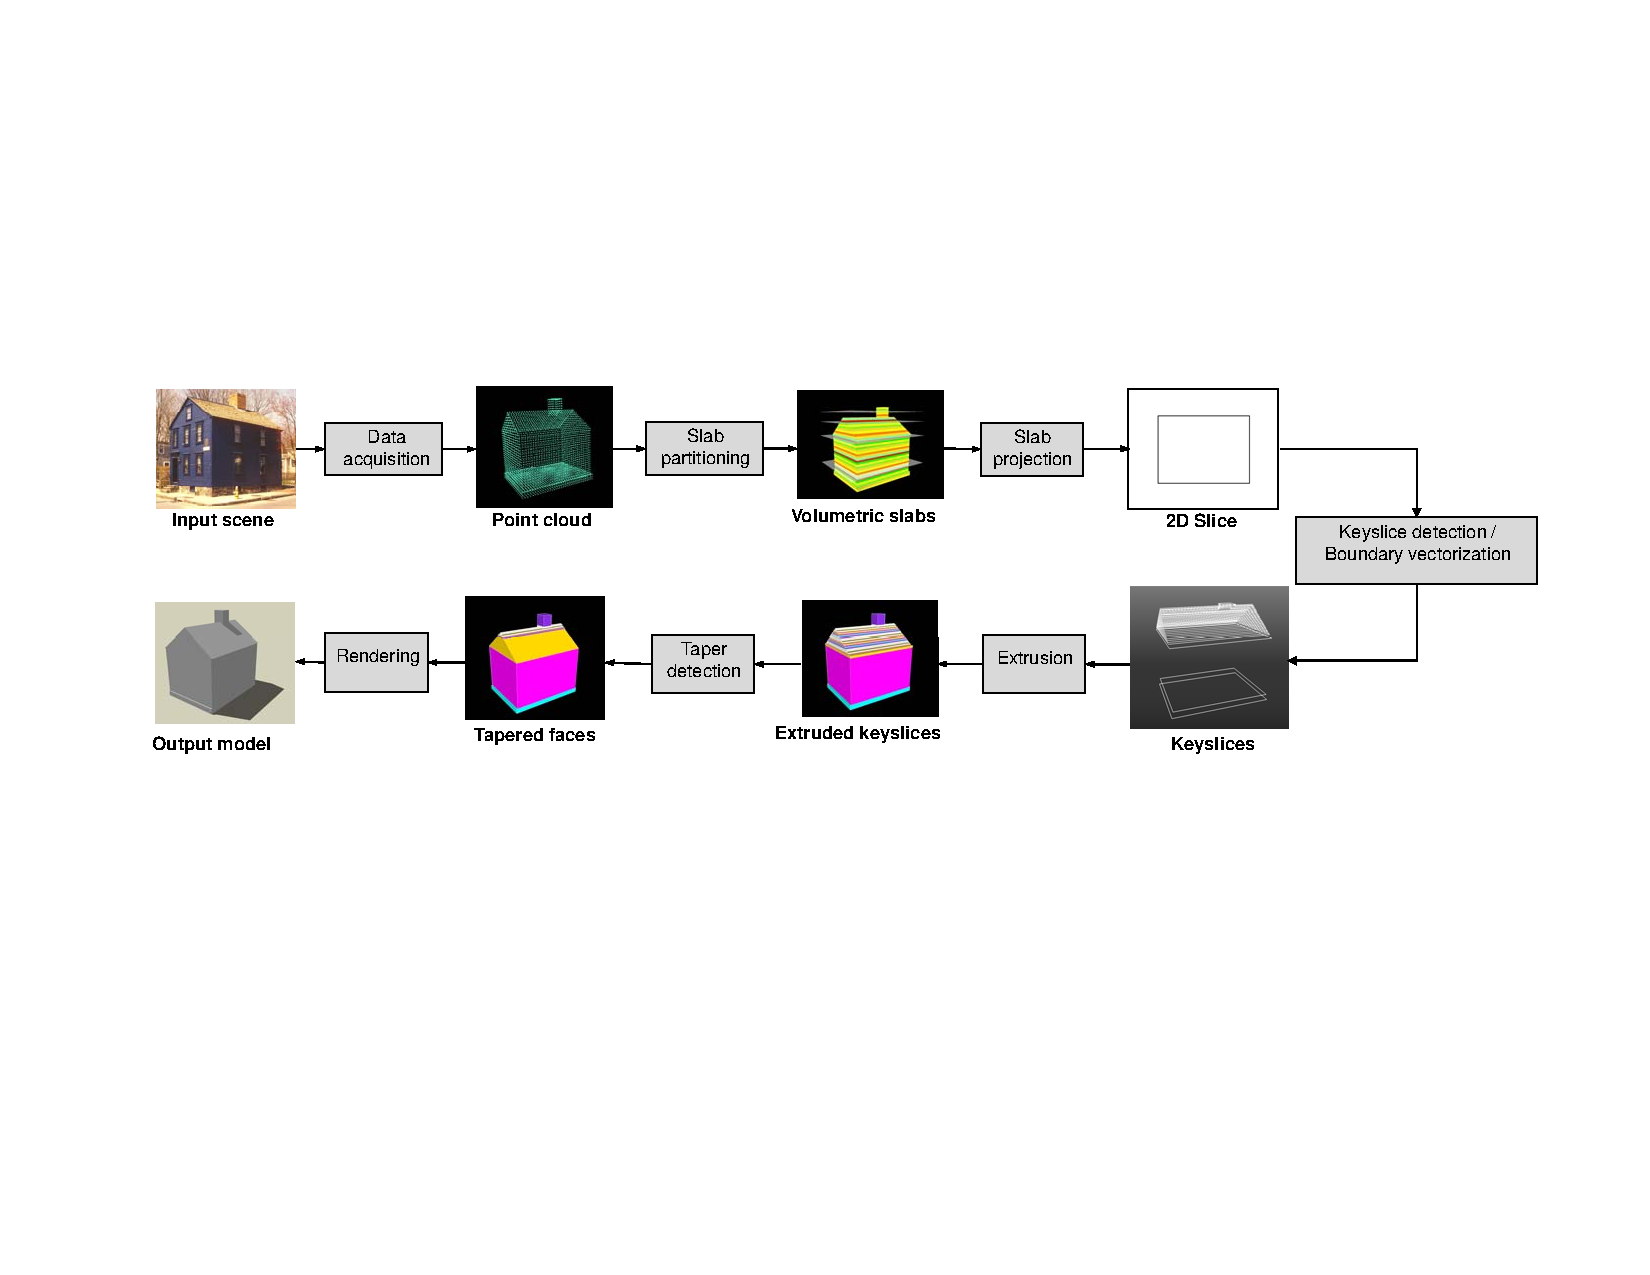
\includegraphics[width=7in]{overview.png}
\end{center}
\caption{The overview of the proposed approach.}
\label{fig:ov}
\end{figure*}
%%% End of Figure

In an attempt to steer clear of tedious and expensive hand-made models,
procedural modeling of buildings in \cite{PMB_MWH,PMB_WWS,PMB_PM} has been proposed.
By using an effective description language, buildings and streets of a virtual
city can be generated automatically.
The strength of this approach is that the description language can generate
a huge number of buildings and streets quickly and beautifully.
This is particular useful for gaming or other computer graphics applications.
However, since the parameters used to generate the buildings are randomly
generated, the city generated with these buildings and streets is a virtual one.
This approach is not useful for attempting to model an {\it existing} building.
In order to do so, one has to manually specify the parameters of the building,
which is very cumbersome.
Our goal is to automatically infer the contours and extrusion/taper parameters
of an existing building directly from dense range data.

There has been a great deal of related work on 3D modeling in the research
community.
Essentially, this modeling process is the reverse engineering problem
of computer graphics \cite{RE_Fisher,RE_CLF,RE_CD}.
Reverse engineering of range data has been applied in numerous research areas,
including computer-aided design (CAD), computer vision, architectural modeling,
and medical image processing.
In \cite{DP_OWYC}, Or et al. proposed a 3D building reconstruction from a 2D floorplan image.
With the help of 2D
floorplan image, both the interior and exterior of a building are reconstructed accordingly.
However, the unavailability of 2D floor plan makes this approach not applicable to most applications,
including our project.
In \cite{RE_TOGSH}, Thompson et al. made use of known manufacturing features
to infer the 3D structure of the mechanical parts.
Their method benefits from the domain knowledge that most of the mechanical
parts consist of predefined structures, such as holes, bosses, and grooves.
Our work is partially motivated by this idea since it also incorporates
{\it a priori} knowledge about the construction of urban buildings for further
inference.
However, their method is based on predefined simple geometry structures and
the assumption that the input 3D data has no holes.
This hinders their approach for those applications with incomplete data.

Multimodal data fusion is an active research direction on large-scale urban environment modeling.
In \cite{UM_Zakhor,UM_HYN}, both air and ground data are fused, including laser scans, camera images,
and aerial images. The LIDAR scans are used to create
the models and the camera images are used for texture mapping.
Xiao et al. \cite{UM_XFTQ} tried to bypass the above tedious data collection process by
proposing a image-based facade modeling of streets, in which they tried to obtain
3D point clouds based on structure from motion (SFM).
All these methods can only partially model the buildings since the 3D information they obtained are far away
from complete, not to metion modeling inside structures of buildings.
Ball-pivoting algorithm (BPA) \cite{BPA_BMRS} is an efficient 3D modeling technique on range data, which might be
the most related work to our proposed method. However, the models it generated require numerous amount
of space for storage, which hinder its capacity on web-based applications. Although the model
generated by BPA could be simplified using some approximation techniques, such as qslim in \cite{BPA_GH},
the sharpness of the original model is not preserved.

We propose an efficient way to reconstruct 3D models from range data by
partitioning the data into thin cross-sectional slabs of volume.
For each slab, all range data in that slab is projected onto a 2D
cross-sectional image slice.
Producing this array of slices permits us to avoid direct computation on
3D data, which is time-consuming and computationally complex.
A similarity measure \cite{IR_Brown} can be used to cluster the sliced images
together into {\it keyslices}.
This term is analogous to ``keyframes'' in computer animation, which denote
important snapshots in the animation sequence from which intermediate results
can be derived.
In essence, each keyframe is a slice in the spatiotemporal volume of
an animation.
Similarly, each keyslice is a 2D image which contains a {\it transitional}
cross-section of the building, encapsulating major changes in the facade.
The model is then generated by applying basic extrusion and taper
operations from one keyslice to the next.
This produces a lightweight representation consisting of only a few
hundred polygons.

%%%%%%%%%%%%%%%%%%%%%%%%%%%%%%%%
%%%%%%   Overview  %%%%%%%%
%%%%%%%%%%%%%%%%%%%%%%%%%%%%%%%%
\section{Overview}
Our approach is schematized in \Fig{ov}.
First of all, the coordinates of the 3D point cloud stored in ascii format are loaded into memory.
To carry out lightweight process, the 3D point data
is projected to a serial of 2D image slices to avoid computation on 3D data directly.
Due to the occlusion and some special structures of the building, such as windows, the input data
is not complete and contains outlier noise.
Therefore, the noise removal and missing data recovering are carried out as a pre-processing stage to
generate the 3D model.
The next stage of the approach is to carry out lightweight
image processing techniques on the enhanced image slices.
As mentioned before, the goal is to reconstruct the 3D
model from the point cloud based on the extruded and tapered
operation. Extrusion detection will cluster the above 2D slices into keyslices, which will
be used for further modeling processing.
After this, boundary vectorization for these raster
keyslices will be conducted. Tapered structure detection is carried out to
further reduce the model size.
For the final 3D model generation and visualization purpose, the inferred 2D information will
be transformed back to 3D world coordinate system, which is the last stage of the proposed approach.
Once all the above steps are completed, a 3D models of urban buildings is reconstructed
from its range data.

%%%%%%%%%%%%%%%%%%%%%%%%%%%%%%%%
%%%%%%   PREPROCESSING  %%%%%%%%
%%%%%%%%%%%%%%%%%%%%%%%%%%%%%%%%
\section{Preprocessing the Range Data}
\label{sec:prep}

The input to our system is range data assembled as a 3D point cloud.
Our data is obtained from a Leica Cyrax 2500 laser range scanner \cite{RDP_LRS},
which works by sweeping an eye-safe laser beam across the scene to collect
up to one million 3D depth points per frame.
All scene points that lie within 100 meters can be acquired with an accuracy
of 5mm in depth.
The basic algorithm that we use for registering the voluminous 3D data
acquired from multiple scans of buildings has been introduced in
\cite{RDP_LS}.
That same algorithm is also responsible for extracting the major axes
of the building in order to align it to the axes of the world coordinate
system.
This is necessary to properly infer the keyslices.
\Figa{IR_2_DXF} displays a properly aligned, {\it registered} 3D point cloud
consisting of 14 scans totalling 14 million points.

Due to occlusions and limited vantage points, the point cloud collected by the
laser scanner contains artifacts and missing data.
In addition, computing directly on 3D data is time-consuming and
computationally complex.
To tackle these issues, we define inner and outer bounding boxes for the
building to clip away unrelated scene objects.
Then, we convert the 3D modeling problem into a set of 2D problems by
projecting the 3D data into a series of 2D cross-sectional images.
Noise removal, hole filling, and vectorization are all done in this
2D space.

\subsection{Extraction of 2D Slices}
\label{sec:image_slicing}
We consider the point cloud data as a large array of 3D points that can be
sliced into horizontal slabs of volume.
All 3D points within each slab will be projected onto a horizontal cutting
plane, or slice, at the base of the slab.
\Fig{slice_slab} shows the 3D point cloud in \Figa{IR_2_DXF} partitioned into 50 slabs.
The 2D cross sections associated with the four displayed cutting planes
are shown in \Fig{slicing}.

\begin{figure} [htbp]
\begin{center}
\begin{tabular}{cc}
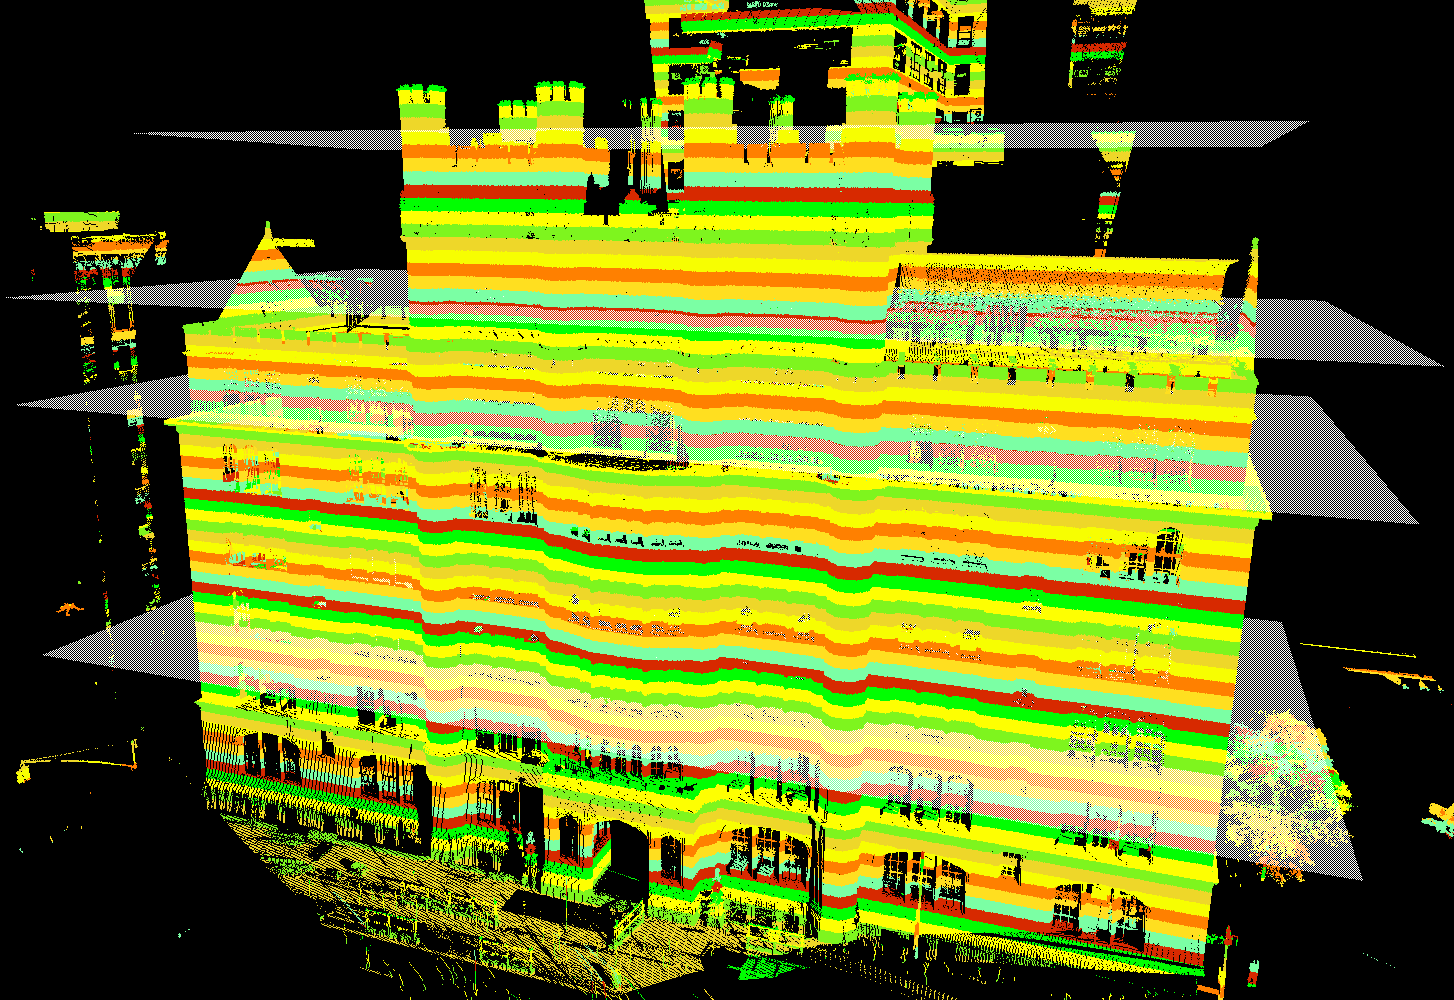
\includegraphics[width=0.4\textwidth]{slab_planar.png}
\end{tabular}
\end{center}
\caption{A set of keyslices from the 3D point cloud in \Figa{IR_2_DXF}.}
\label{fig:slice_slab}
\end{figure}

The height of each slab is $\boldsymbol{\delta}$.
If that value is held constant, each slice is generated from equal-sized
slab intervals.
If $\boldsymbol{\delta}$ is allowed to vary, then we may
choose to allow for large values in parts of the structure that are similar,
and low values in regions that contain finer detail.
To avoid working on 3D data directly, a relatively small constant value
for $\boldsymbol{\delta}$ is chosen to generate 2D cross-sectional image slices.

\begin{figure} [htbp]
\begin{center}
\begin{tabular}{cc}
\fbox{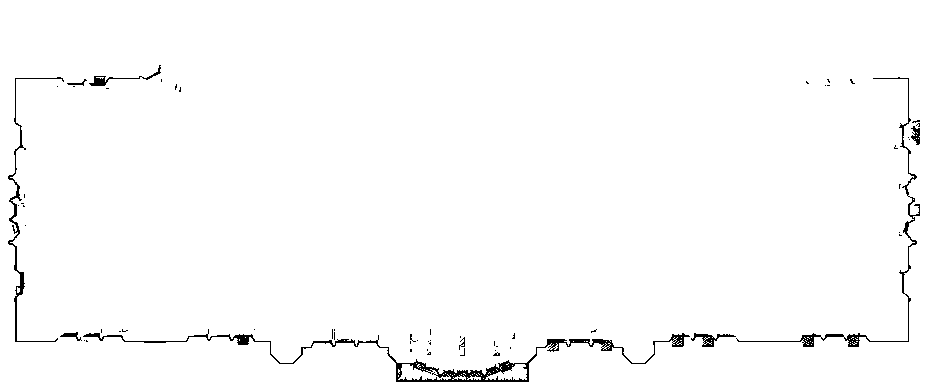
\includegraphics[width=0.2\textwidth]{image_slice_0190.png}} &
\fbox{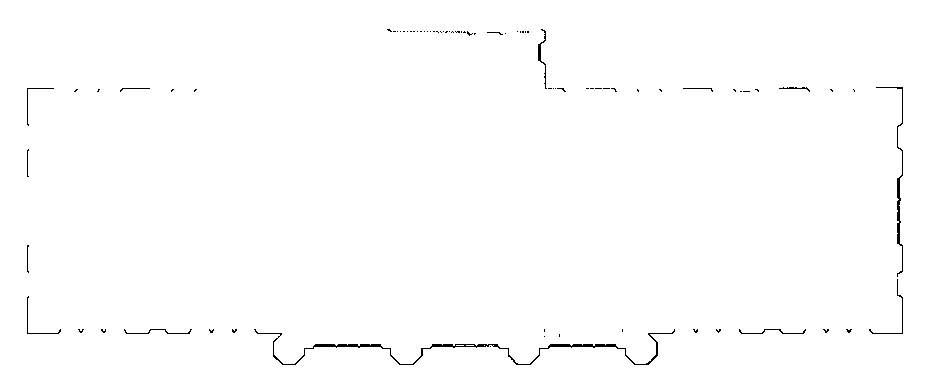
\includegraphics[width=0.2\textwidth]{image_slice_0600.png}} \\
(a) & (b) \\
\fbox{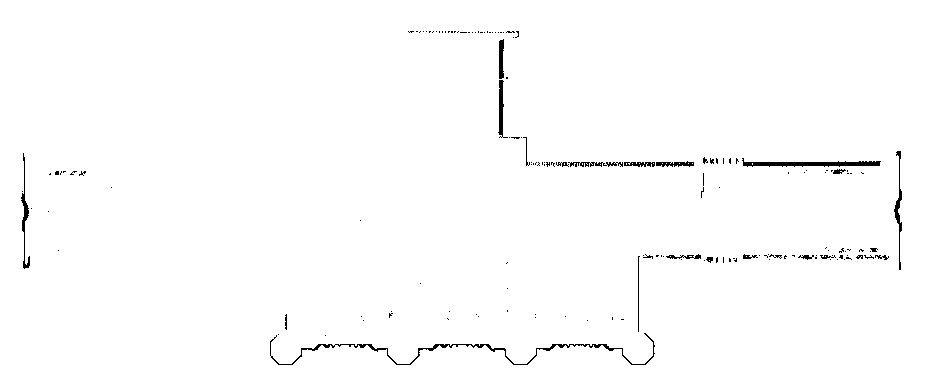
\includegraphics[width=0.2\textwidth]{image_slice_0714.png}} &
\fbox{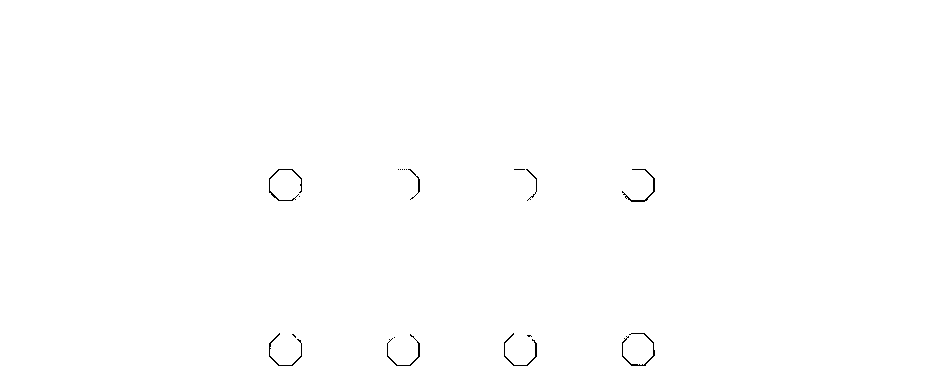
\includegraphics[width=0.2\textwidth]{image_slice_0951.png}} \\
(c) & (d)
\end{tabular}
\end{center}
\caption{A set of keyslices from the 3D point cloud in \Figa{IR_2_DXF}.}
\label{fig:slicing}
\end{figure}

Without loss of generality, the $y-$axis is used to represent the bottom-up
vertical direction.
We project the 3D data
$\boldsymbol{P}(x,y,z), H_{lo} \leq y < H_{hi}$, in the height range
$[H_{lo}, H_{hi})$ onto a 2D image slice.
The projection is normalized in the range $[0,W]$,
where $W$ is the image width:
\begin{equation}\label{eq_image_slicing}
[\,x^{2D},\; y^{2D}\,]^T = \omega\cdot[\,x^{3D}_i - X_{MIN},\; z^{3D}_i - Z_{MIN}\,]^T
\end{equation}
Note that $\omega = W/(X_{MAX} - X_{MIN})$, and that
the [$X_{MIN}$, $X_{MAX}$] and [$Z_{MIN}$, $Z_{MAX}$] pairs define the
3D bounding box, which can be obtained through user input and can be used
to clip away noise data.
\Fig{slicing}(a)-(b) show some examples of the 2D slices, where noise
and incomplete data are observed.

\subsection{Missing Data Recovery}
\label{sec:mdr}
The slices we extract above often have holes due to occlusion or other
visibility issues.
Fortunately, most urban buildings have symmetry that we can exploit to
fill these holes.
Symmetry computation on 3D data \cite{Sym_PSGRF,Sym_ZPA} is expensive,
so we conduct this computation on the 2D image slices.
Since the 3D data has been already rectified \cite{RDP_LSYGS} and projected onto 2D slices, hence only 2D translation
is needed to be considered for symmetry computation.
Let $P(x,y)$ be a point on the original image $I$ and $P'(x',y')$ be the reflected
point of $P$ with respect to a symmetry line $L$.
The symmetry computation equation for $L$ is as follows:
\begin{equation}
L = \underset{x,y}{\operatorname{arg\,min}}\sum{d_{x,y}(P', I)}
\end{equation}
where the $d_{x,y}(P',I)$ is the distance between the self-reflected point
$P'$ and its nearest data point in image $I$.
The reflected point $P'$ of the original point $P$ is computed with
respect to a line along either the $x-$ or $y-$ axis.
Therefore, the symmetry line $L$ is obtained as the line with minimum
summation error over the reflected data points.
\Figa{sym} and \Figb{sym} depict the original and missing data recovered with symmetry
computation, respectively.
%%% Figure of the tapered template.
\begin{figure}[htbp]
\begin{center}
\begin{tabular}{cc}
\fbox{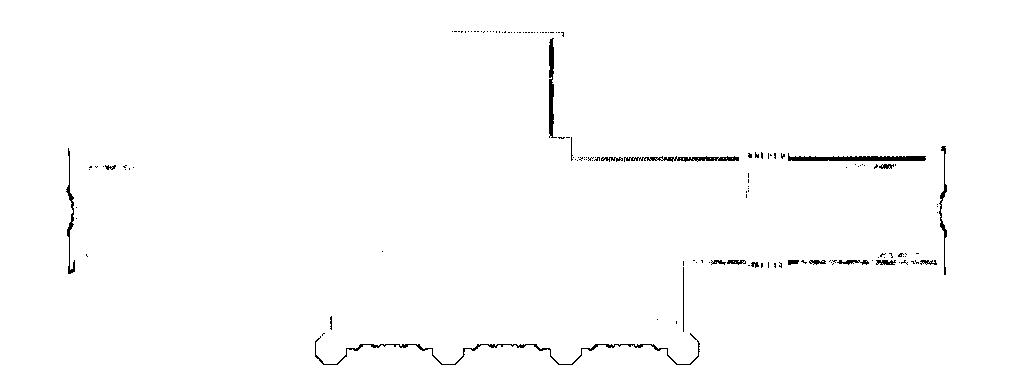
\includegraphics[width=0.2\textwidth]{image_slice_0705_0711.png}} &
\fbox{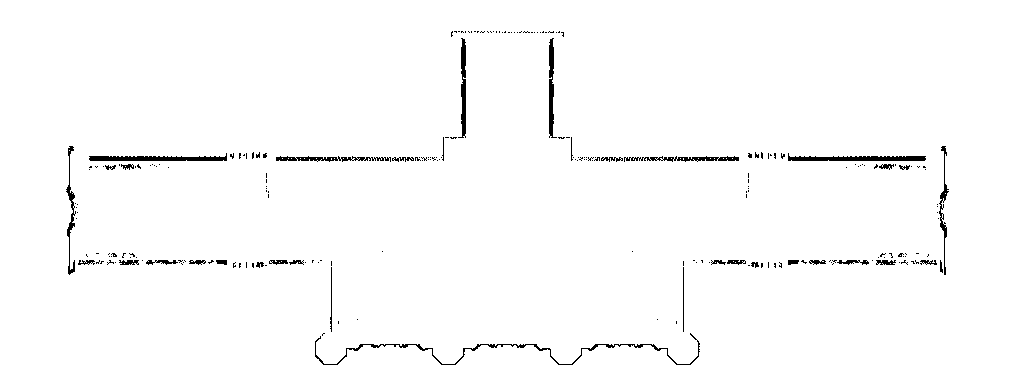
\includegraphics[width=0.2\textwidth]{image_slice_0705_0711_recoverd.png}} \\
(a) & (b)
\end{tabular}
\end{center}
\caption{ Symmetry based missing data recovery. (a) original 2D slice image (b) Recovered image.}
\label{fig:sym}
\end{figure}
%%% End of Figure


%%%%%%%%%%%%%%%%%%%%%%%%%%%%%%%%
%%%%%%   3D Reconstruction  %%%%
%%%%%%%%%%%%%%%%%%%%%%%%%%%%%%%%
\section{Lightweight 3D Reconstruction}
\label{sec:reconst}
Our 3D modeling algorithm is based on \emph{a priori} knowledge that
urban buildings can be created through a series of extrusion and taper
operations on the salient cross-sections contained in the keyslices.
It is therefore critical to identify those salient cross sections upon
which the extrusion and taper operations will apply.
This will be the key step for successful modeling.

\subsection{Extrusion Detection}
\label{sec:ksd}
The 2D image slices of an extruded region are similar to each other.
Thus, to detect an extrusion region one only needs to compute
the similarity between adjacent slices.
The Hausdorff distance is chosen here as the similarity measure.
Let $P_r(x_r, y_r)$ be a data point in a reference image and
let $P_i(x_i, y_i)$ be a data point in a new observed image $I$.
The Hausdorff distance of image $I$ to reference image $I_r$ is defined as:
\begin{equation} \label{eq.hd}
d_H(I, I_r) = \sum_{i=0}^Nd_{min}(P_i, I_r)
\end{equation}
where $d_{min}(P_i, I_r)$ is the minimum distance from data point $P_i$
in image $I$ to the reference image $I_r$.
Alternatively, we can also define the Hausdorff distance, $d_H(I_r, I)$,
from reference image $I_r$ to a new observed image $I$, using the equation \ref{eq.hd}.
These two distances are usually not equal to each other.
As a rule of thumb, one can choose
$d_{HD} = \text{MAX}\{d_H(I, I_r), d_H(I_r, I)\}$ as the Hausdorff distance.
To compute the keyslices, a threshold $\tau_{d}$ is used for the
Hausdorff distance $d_{HD}$.
If $d_{HD} < \tau_{d}$, the two images $I$ and $I_r$ are considered
similar to each other.
Otherwise, a keyslice image is found and $I_r$ is updated with $I$,
the new keyslice image.

The accuracy of the keyslices detected by using the Hausdorff distance
is mainly dependent on the threshold $\tau_d$.
Small $\tau_d$ leads to more accurate models and will require more time and
space to compute and store the result.
Therefore, there is a trade-off between model accuracy and time-space
efficiency.
This leads to an issue that when the threshold $\tau_d$ is relative large
in order to keep the time and space efficiency, some potential keyslices which
contain salient structure may be missed.
To conquer this problem, the curvature information is computed as a complementary
criteria for the keyslice detection.

This idea is based on the observation that the keyslices are generally
located at the curvatures observed from the boundary of 2D slices extracted
at orthogonal direction. \Fig{HT_BPA_Curvature} shows such a 2D slice in the left.
In the right close-up view of a small region, two curvatures, $c_1$ and $c_2$, are
computed in this small region. The red, blue and green lines indicate the locations
of the center, the starting and the ending of a curvature. 
As a matter of fact, there is a third curvature computed around the
black box sitting on top of the green line of the curvature $c_1$. 
However, this third one should not be consider as a real curvature 
in that the black box is due to an air conditioner during the data acquisition process, 
which means it is not a part of the building. We called this third curvature
{\it outlier curvature} which needs to be removed from the set of real curvatures.
Based on the fact that these outlier curvatures exist only in a few 2D slices,
we can exclude them by counting the number of appearance for each curvature.
Only those curvatures appears in most of the 2D slices are kept for further computation.

%%% Figure of the tapered template.
\begin{figure}[htbp]
\begin{center}
\begin{tabular}{c}
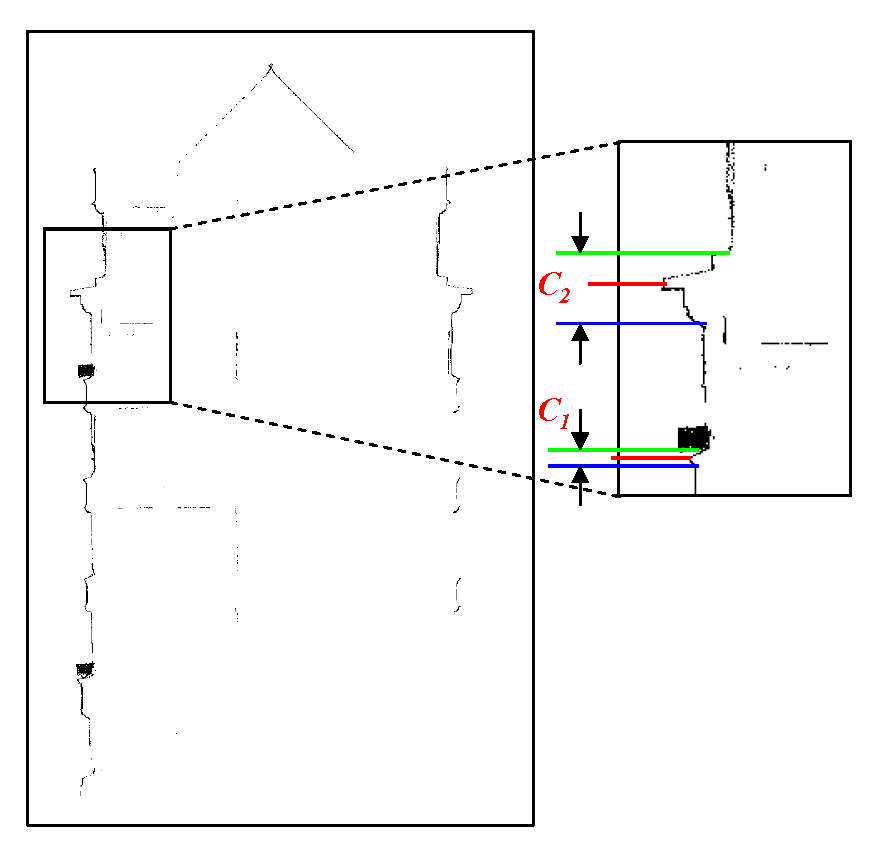
\includegraphics[width=0.35\textwidth]{curvature.pdf}
\end{tabular}
\end{center}
\caption{ Curvature based key slice detection. }
\label{fig:HT_BPA_Curvature}
\end{figure}
%%% End of Figure

Once the real curvatures are obtained, they can be used as a complemental way of 
Hausdorff distance for keyslices detection. 
Each curvature $c$ is mapped to a set $s$ of original 2D cross-sectional
slices, $i,\ldots,j$, where $i$ and $j$ are corresponding to the starting and 
the ending locations of $c$. After this, the set $s$ is checked whether 
it contains any keyslice or not.
If a keyslice $k$ has been marked in $s$ by Hausdorff distance, 
nothing needs to be done and this curvature $c$ is discarded. 
On the other hand, if $s$ contains no keyslice, $i$ and $j$ will be marked as 
two new keyslices to keep the salient feature identified by this curvature $c$.
The combination of Hausdorff distance measurement and curvature inference
ensures that the salient structures of a building will be preserved.


\subsection{Boundary Vectorization}
\label{sec:BPA}
After the keyslices are detected, $N_K$ keyslices will be identified
from a total of $N_A$ image slices.
Depending on the threshold $\tau_{d}$, $N_K$ is usually about one to two
orders of magnitude smaller than $N_A$, e.g., $N_K/N_A$ is 0.06 when
$\tau_d$ = 4.0 for the example in \Figa{IR_2_DXF}.
To generate the 3D model, these keyslice images need to be vectorized to
represent the silhouette or boundary of the building.
Several raster image vectorization approaches are proposed in
\cite{DP_AAKMT,DP_DP}.
The Douglas-Peucker algorithm attempts to connect all of the existing points
to form a polygon.
Although the implementation of this approach is very efficient with the
improvement described in \cite{DP_HS}, this method cannot handle the case
where spurious interior points are present, which contributes to outlier data.
To tackle this issue, we adapted the ball-pivoting algorithm (BPA)
\cite{BPA_BMRS} from its original use on 3D point cloud data to use on
2D keyslice images where it produces vectorized boundaries.
The key parameter for the BPA algorithm to work successfully is to
find the right size of the ball for pivoting.
We propose a coarse-to-fine adaptive BPA algorithm, described below,
to solve this problem.

\begin{figure}[hbtp]
\centering
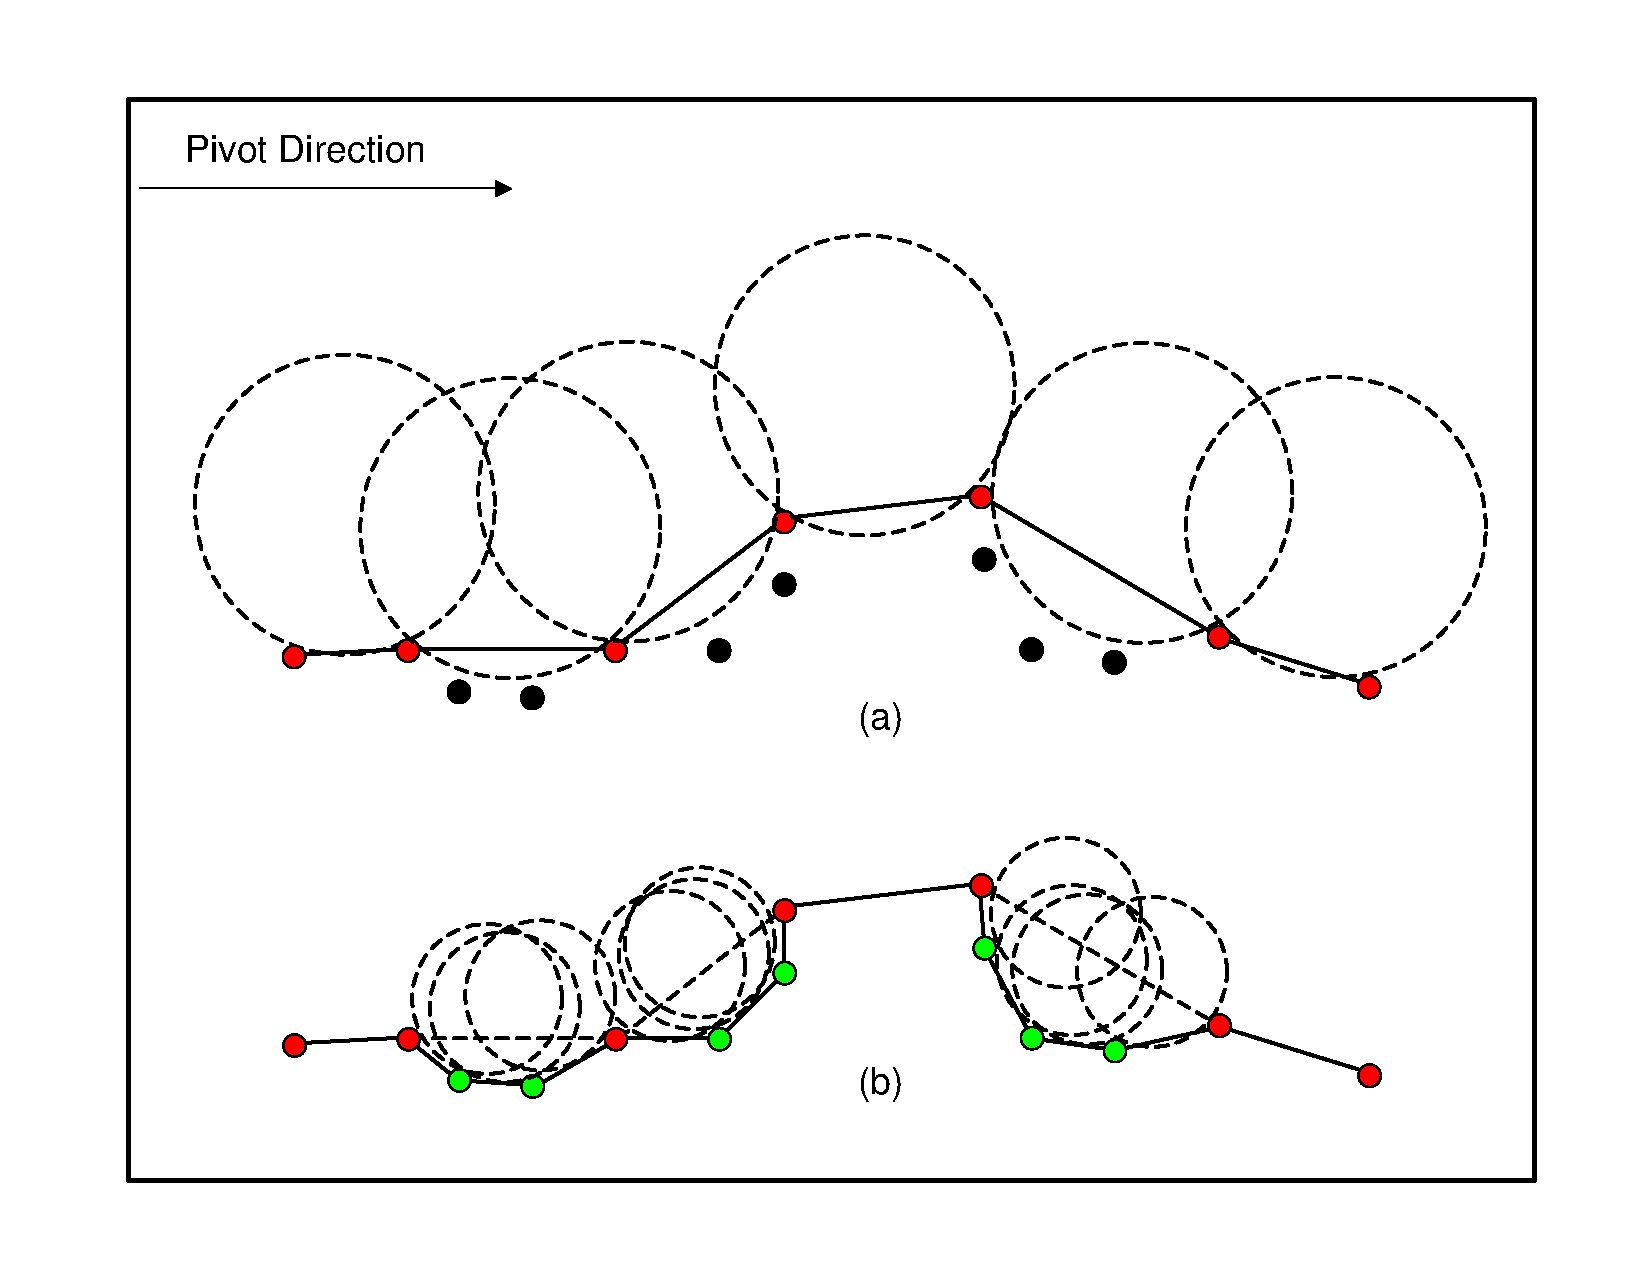
\includegraphics[width=0.4\textwidth]{figures/BPA.pdf}
\caption{Ball pivot algorithm: (a) Initial pivoting with circle of radius 2$r$;
(b) Refinement process with circle of radius $r$.}
\label{fig:BPA}
\end{figure}

Due to the gap between data points, a relatively large radius $r$ is chosen
as a coarse step to ensure that the ball will travel across all boundary
data before turning back or reaching any existing boundary points.
\Figa{BPA} shows an initial ball-pivoting process on 2D data points.
The output of the initial BPA $\boldsymbol{\Phi}$ contains an ordered list of the boundary data
points $\boldsymbol{P}$ and their corresponding directions $\overrightarrow{\boldsymbol{R}}$ in which
the circle $C$ starts pivoting.
The iterative BPA refinement process is applied on $\boldsymbol{\Phi}$ to get more accurate results with
a smaller radius $r'=r/2$ as shown in \Figb{BPA}.
The length of each line segment formed by adjacent points
is checked, $\ell = \overline{P_0P_1}$, in $\boldsymbol{\Phi}$.
If this line is long enough, the BPA is applied between the two adjacent points.
When the ball reaches the second point, a new list of ordered boundary points,
$\boldsymbol{\Phi'}$, is inserted into $\boldsymbol{\Phi}$ between $P_0$ and $P_1$.
This process continues until it finishes checking every adjacent point in $\boldsymbol{\Phi}$.
The refinement stops when $r'$ falls below threshold $\tau_r$.

%%% Adaptive BPA + HT %%%%

Although the adaptive BPA is a very efficient and straight-forward approach to vectorize
the boundary or silhouette of raster images, it produces a lot short line segments and
is prone to the noise. This is illustrated
in \Figa{HT_BPA_figure}. As we can see, the upper part of the vectorized image
contains some bogus detailed structures which actually belong to the same line structure. In the
case where the outlier is not close enough to the real data, the result will be significantly
degraded. Based on the observation that most of the boundaries of the man-made building
are of line structures, we can improve the adaptive BPA results by incorporating the line
information.

%%% Figure of the contours
\begin{figure}[htbp]
\begin{center}
\begin{tabular}{cc}
\fbox{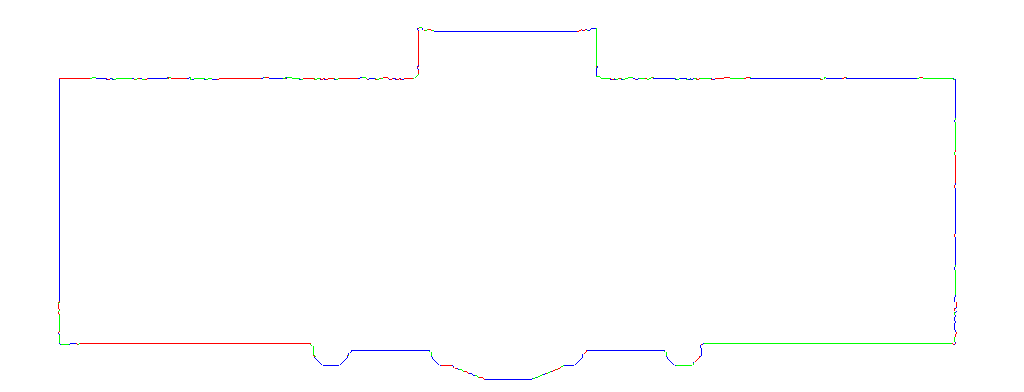
\includegraphics[width=0.2\textwidth]{bbb_image_slice_1024_392_0533_refine_with_rad_1_and_merged.png}} &
\fbox{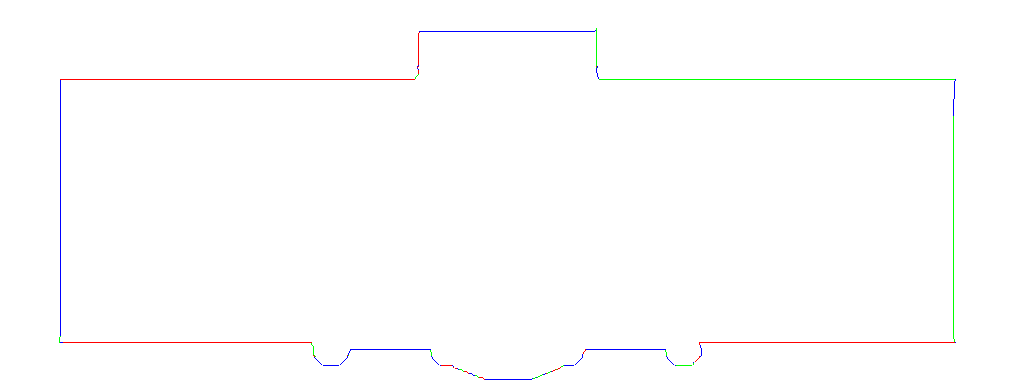
\includegraphics[width=0.2\textwidth]{bbb_image_slice_1024_392_0533_combine_HT_BPA_rad_32.png}} \\
(a) & (b)
\end{tabular}
\end{center}
\caption{  (a) a sliced image vectorization with adaptive BPA
(b) the combination of hough transform and BPA on the sliced image.}
\label{fig:HT_BPA_figure}
\end{figure}
%%% End of Figure

To combine the adaptive BPA with HT, we first apply our adaptive HT algorithm on the raster
image to obtain all lines $\boldsymbol{L}$ and sort them from the longest to the shortest one.
Generally speaking, the longer lines give more confidence on the line structure of the building.
For integration, we first apply dilation operation on $I$ using 8-connected kernel
to get the dilation image, $I_d$. The next step is to measure how well the lines in
$\boldsymbol{L}$ match the data in $I_d$, which determines whether a line in $\boldsymbol{L}$
should be used as a substitution or not.

If a line segment $L$ is found to be a good candidate, the next step is to find the corresponding part of the
BPA points in $\boldsymbol{\Phi}$ for substitution. To do this, we first compute the closest two points
$P_i$ and $P_j$ in $\boldsymbol{\Phi}$ to the two end points of $L$.
Generally speaking, the points in $\boldsymbol{\Phi}$ represent a polygon and therefore form a circle layout, i.e.,
$\boldsymbol{P} = \{ P_0,P_1,\ldots ,P_{n-1}, P_0 \}$. Assume $i < j$, there are two possible choices to replace
the series of the points, which are
$\boldsymbol{P_1} = \{ P_i,P_{i+1},\ldots,P_{j-1}, P_j \}$, and
$\boldsymbol{P_2} = \{ P_j,P_{j+1},\ldots,P_{i-1}, P_i \}$.
To determine which one is correct, one can compare the distance, $D$, from the line $L$ to both
set of the points $\boldsymbol{P_1}$ and $\boldsymbol{P_2}$. The point set with smaller $D$ is
about to be substituted by the line $L$.
\begin{equation*}
D = \underset{\boldsymbol{P_1},\boldsymbol{P_2}}{\operatorname{arg\,min}}\sum{\lVert P_i - L \rVert}
\qquad P_i \in \boldsymbol{P_1} \ \text{or} \ P_i \in \boldsymbol{P_2}
\end{equation*}
where $\lVert P_i - L \rVert$ is the Euclidean distance from a point $P_i$ to the line $L$.

After being replaced with line structures detected by Hough transform, the beautified contour is
shown in the \Figb{HT_BPA_figure}. As we can see, the top part of the contour which was consisting
of those short line segments were replaced two line segments, which make the contour simpler and neat
for modeling.

\subsection{Tapered Structure Detection}
\label{sec:tsd}
After the keyslices are detected and vectorized, the silhouettes of
$N_K = \{I_{i}, i = 0, ..., K \}$ keyslices
can be used to represent the whole building based on the extrusion operation.
That is, the space between each pair of keyslices, say $I_{i}$ and $I_{j}$,
can be interpolated by the lower keyslice, e.g., $I_{i}$ in this case.
This is valid due to the similarity between the intermediate images and the
keyslice $I_{i}$.
By modeling a building using this series of keyslices $N_K$, we can largely
reduce the space needed to store urban buildings.
This helps make possible 3D web-based applications such as 3D city navigation.

%%% Figure of the tapered template.
\begin{figure}[htbp]
\begin{center}
\begin{tabular}{c}
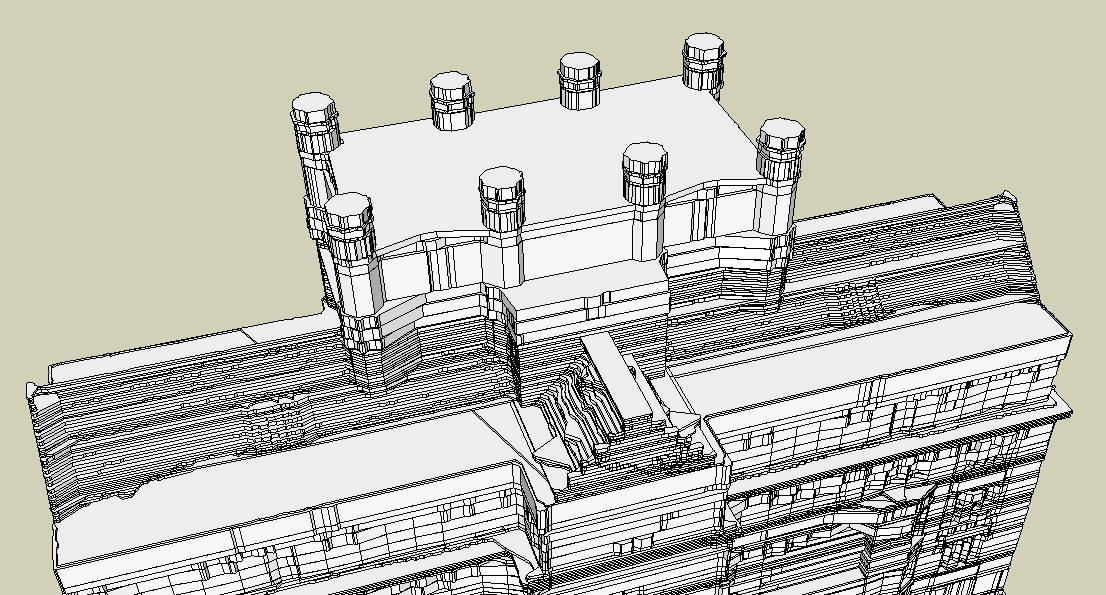
\includegraphics[width=0.35\textwidth]{extrude_1.png} \\
(a) \\
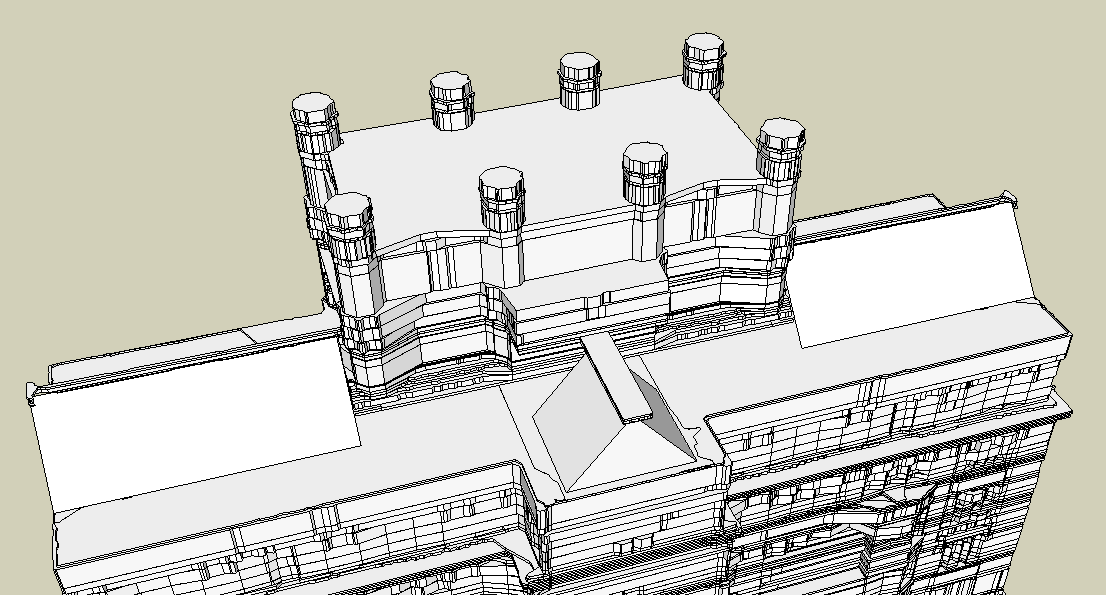
\includegraphics[width=0.35\textwidth]{extrude_2.png} \\
(b)
\end{tabular}
\end{center}
\caption{The top view of the 3D building. (a) without tapered structure. (b) with tapered structure.}
\label{fig:DXF_top}
\end{figure}
%%% End of Figure

In addition to the extrusion operation, we can further improve the model
and reduce the model size by observing that part of the keyslice images
belong to the same tapered structure, as demonstrated in \Fig{DXF_top}.
\Figa{DXF_top} shows the roof structure
of the reconstructed model based on a keyslice image extrusion operation with
almost half of the keyslice images dedicated to the structure.
After applying the tapered structure inference, \Figb{DXF_top}
shows the improvement of the modeling, which is much smoother than the
previous model.
In addition, the keyslices needed to represent the building, and its
associated storage, are reduced almost in half.

The difficulty of inferring tapered structure lays on the complication of
the building structure itself.
Let's assume that the height range for roof structure is
$H_R = [H_{lo}, H_{hi}]$.
If this is the only existing structure between $H_R$, it is simple and
straight-forward to detect and infer this part.
%Namely, we only need to find the corresponding feature points between the bottom
%the top feature points.
However, for some complicated structures, such as a mixed layout
of tapered and extruded structures as depicted in \Fig{taper_seg},
 some special treatment is needed to obtain the desired results.
Our approach is based on the divide and conquer strategy: the whole
structure $\boldsymbol{U}$ is segmented into independent sub-structures,
$U_0, U_1, \ldots, U_N$. For any sub-structure $U_i$,
it contains only a unique structure, either a tapered or an extruded one. Once
each unit $U_i$ is inferred, the whole structure can be modeled by an union operation
of these sub-structures, i.e., $\boldsymbol{U} = \bigcup{U_i\{ i = 1,\ldots,N\}}$.
Before segmentation, the potential height ranges $H_R$ containing the tapered structures should be computed.
This can be done by checking the frequency of the keyslice images.
The structure containing tapered sub-structures will show a high and even
distributed keyslice images. This is a very useful clue for $H_R$ detection.

%%% Figure of the tapered template.
\begin{figure}[htbp]
\begin{center}
\begin{tabular}{cc}
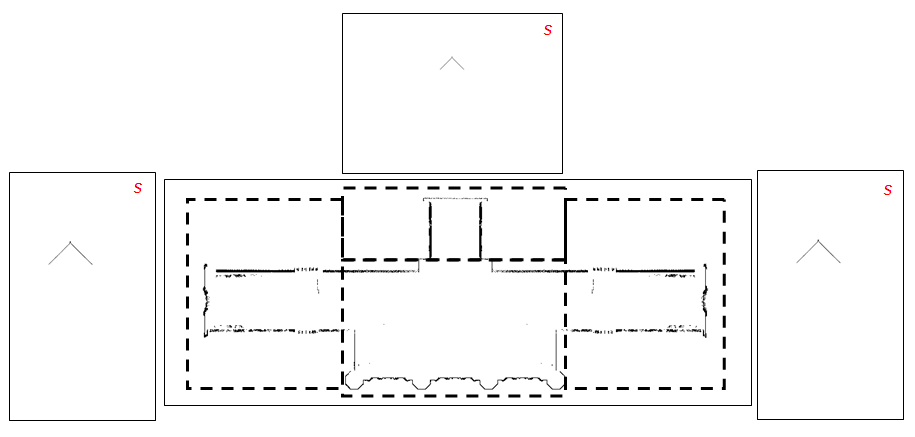
\includegraphics[width=0.45\textwidth]{extrude_3.png} \\
\end{tabular}
\end{center}
\caption{The top view of the 3D building. }
\label{fig:taper_seg}
\end{figure}
%%% End of Figure

Once the potential height ranges $H_R$ is obtained,
the next step is to segment the whole structure $\boldsymbol{U}$ between $H_R$ into
sub-structures, $U_i, \; i = 0,\ldots,N$. This is again done by similarity measurement of sliced images
from orthogonal directions. As before, the 3D data points following inside the range of $H_R$
are projected along both left-right ($X$ axis) and face-inside ($Z$ axis) directions.
Then the keyslice detection is carried out based on Hausdorff distance similarity measurement for
both directions. These keyslices will segment the structure in $H_R$ into sub units of $U_0, U_1, \ldots, U_N$.

For each sub unit $U_i$, we have to know whether it represents an extruded or a tapered
structure. The method is to check in the keyslice image $I_k$ of $U_i$ whether there exists
a pattern where two lines intersect with some appropriate angle.
% as shown in \Fig{TSD_fig_tapered_template}.
If such a pattern exists in $I_k$, such as the images marked with red $s$ in \Fig{taper_seg},
the unit $U_i$ is considered as a tapered sub-structure. Otherwise, $U_i$ is treated as
an extruded sub-structure. If $U_i$ is an extruded unit, its silhouette from the
$y-$ axis is vectorized and is ready for the union operation to obtain $\boldsymbol{U}$.
On the other hand, if $U_i$ is a tapered unit, the bottom and top position have to be computed
so that it can be reconstructed. To do this, all line segments $\boldsymbol{L}$ in $U_i$
are computed using the Hough Transform and the
%described in Algorithm \ref{alg.AHT}.
intersection point $P_0$ of $\boldsymbol{L}$ indicates
the top position of the tapered unit. The other end points $P_i$ of $\boldsymbol{L}$ are also computed
to infer the bottom shape and position.

%%%%%%%%%%%%%%%%%%%%%%%%%%%%%%%%
%%%%%%   Experimental Results%%%
%%%%%%%%%%%%%%%%%%%%%%%%%%%%%%%%
\section{Experimental Results}
\label{sec:IR_OUT}
The results of the extrusion and tapered structures computation,
together with raster image vectorization, are stored in the 2D
image coordinate system. To generate the final 3D model, these
data need to be transformed
back into the 3D world coordinate system.
Let $P(x,y)$ be a point in the 2D image coordinate system, and let
$P'(x,y,z)$ be the 3D world coordinate of $P$, where $y$ is the depth coordinate.
For all points in the same boundary layer or silhouette,
the points lay in the same plane and hence have the same value of $y$.
The equation for transforming $P$ back to $P'$ is a reverse transformation of $\boldsymbol{T_0}$
in the equation \ref{eq_image_slicing}:
\begin{equation}\label{eq_ir2dxf}
[\,x^{3D},\; y^{3D},\; z^{3D}\,]^T = [\,\eta\cdot x^{2D} + X_{MIN},\; \zeta + Y_{MIN},\; \eta\cdot z^{2D} + Z_{MIN}\,]^T
\end{equation}
where $\eta=1/\omega$ and $\zeta=\kappa\cdot\delta$. Here, $\kappa$ is the index of the 2D slice and $\delta$
is the height of a slab described in \Sec{image_slicing}.
\Figd{IR_2_DXF} shows an exterior 3D model generated by the above
transformation.

%%% Figure of the tapered template.
\begin{figure*}[htbp]
\begin{center}
\begin{tabular}{cc}
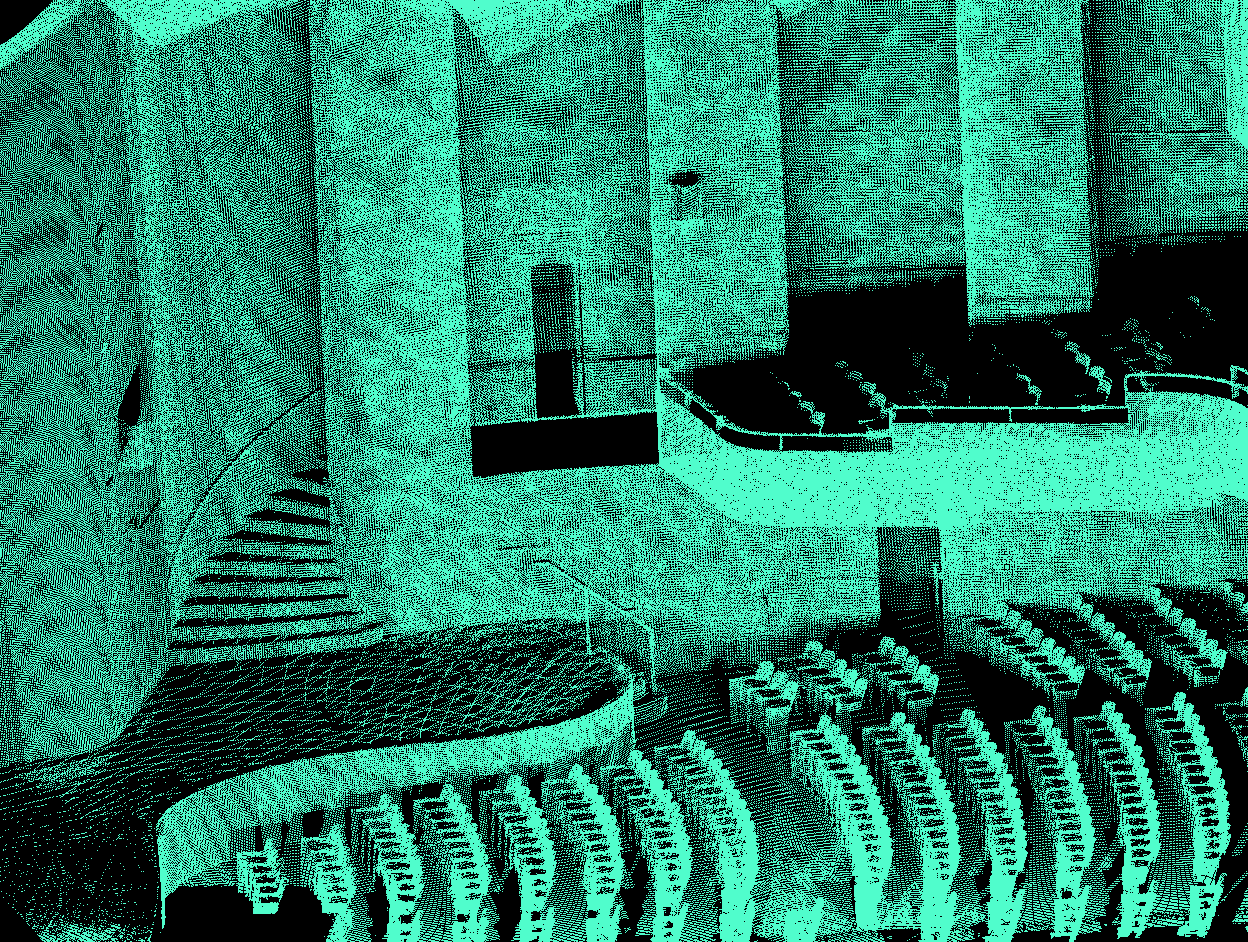
\includegraphics[width=2.5in]{range_crop.png} &
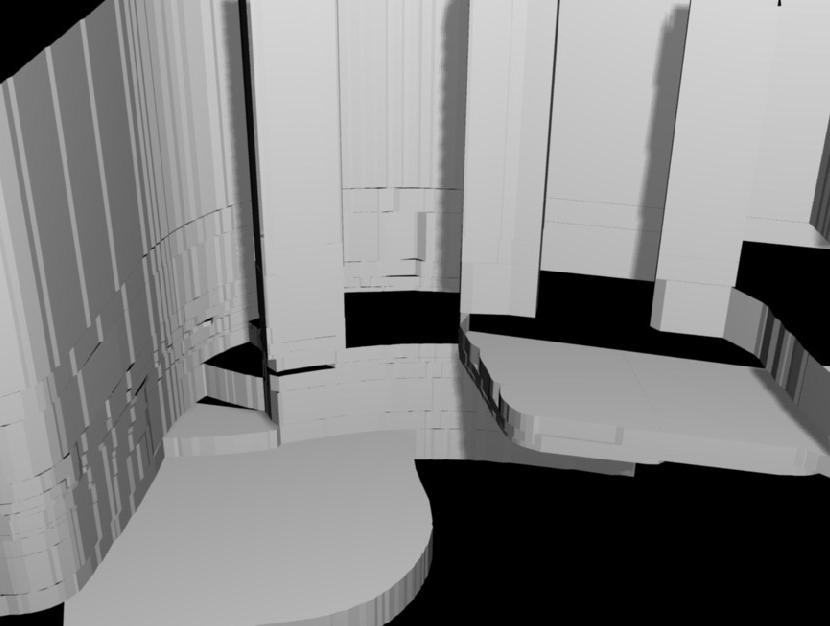
\includegraphics[width=2.5in]{HunterTheatreShaded.jpg} \\
(a) & (b)
\end{tabular}
\end{center}
\caption{The model of an interior scanning. (a) The snapshot of the interior
scanning point cloud data. (b) the model reconstructed from the interior
scanning.}
\label{fig:IN}
\end{figure*}
%%% End of Figure

In addition to the exterior model, we have also applied the approach on
the range data of an interior scanning.
The snapshot of this interior scan is shown in \Figa{IN}
and its reconstructed 3D model is shown in \Figb{IN}.
This model is primarily reconstructed using the extrusion unit, and the
chairs and some fine details are ignored. However, the
main structures of the interior are captured and the chairs can be added to
the model through texture mapping.
Please note that the model generated in \Figb{IN} is of low resolution
and some details may lost, which can be captured by using a smaller
threshold $\tau_d$ to obtain higher resolution models.

\setlength{\tabcolsep}{4pt}
\begin{table}[hbtp]
\begin{center}
\caption{The error measurement with respected to Hausdorff distance threshold $\tau_d$.
The BPA radius threshold $\tau_r = 4$}
\label{tbl_em}
  \begin{tabular}[t]{||c||c|c|c||}
    \hline
    $\tau_{d} $(pixel) & Error (mm)& \# of faces & Size (KB) \\
    \hline \hline
    64 & 0.658 & 1471 & 15\\   %   64 & 9.63 & 1471 & 15\\
    \hline		      %   \hline		
    32 & 0.294 & 3284 & 32\\   %   32 & 4.30 & 3284 & 32\\
    \hline		      %   \hline		
    16 & 0.141 & 8574 & 86\\   %   16 & 2.06 & 8574 & 86\\
    \hline		      %   \hline		
    8 & 0.131 & 13955 & 137\\  %   8 & 1.91 & 13955 & 137\\
    \hline		      %   \hline		
    4 & 0.094 & 27214 & 261\\  %   4 & 1.38 & 27214 & 261\\
    \hline		      %   \hline		
    2 & 0.088 & 31331 & 335\\  %   2 & 1.28 & 31331 & 335\\
    \hline
    1 & 0.083 & 32187 & 337\\  %   1 & 1.21 & 32187 & 337\\
    \hline
  \end{tabular}
\end{center}
\end{table}
\setlength{\tabcolsep}{1.4pt}
To measure the error of a reconstructed 3D model,
we first transform it to the 3D point cloud coordinate system.
The error is measured as the distance from the sampled 3D points to their closest model planes, which
is computed using the following formula:
\begin{equation}\label{eq_em}
E = \frac{1}{|X|}\sum_{x\in{X}}{d^2(x, M)}
\end{equation}
where $X$ is the set of 3D point cloud data. The distance
$d(x, M) = \text{min}_{p \in M}\lVert x - p \lVert$ is the minimum Euclidean distance from
a 3D point $x$ to its closest face $p$ of $M$.

%%% Figure of the tapered template.
\begin{figure} [htbp]
\begin{center}
\begin{tabular}{cc}
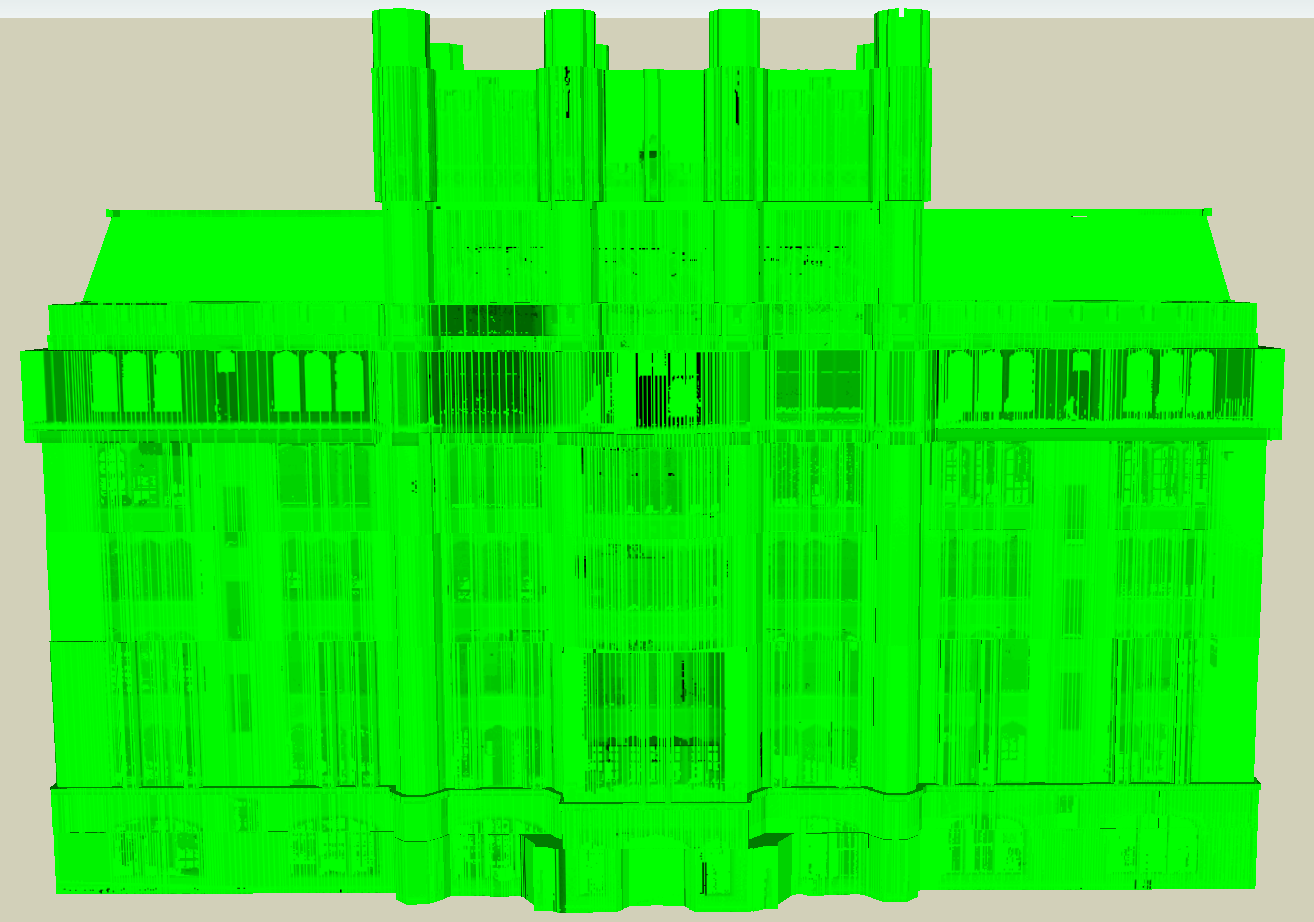
\includegraphics[width=0.2\textwidth]{IR_skp_error_face_1000_32_4_paper.png} &
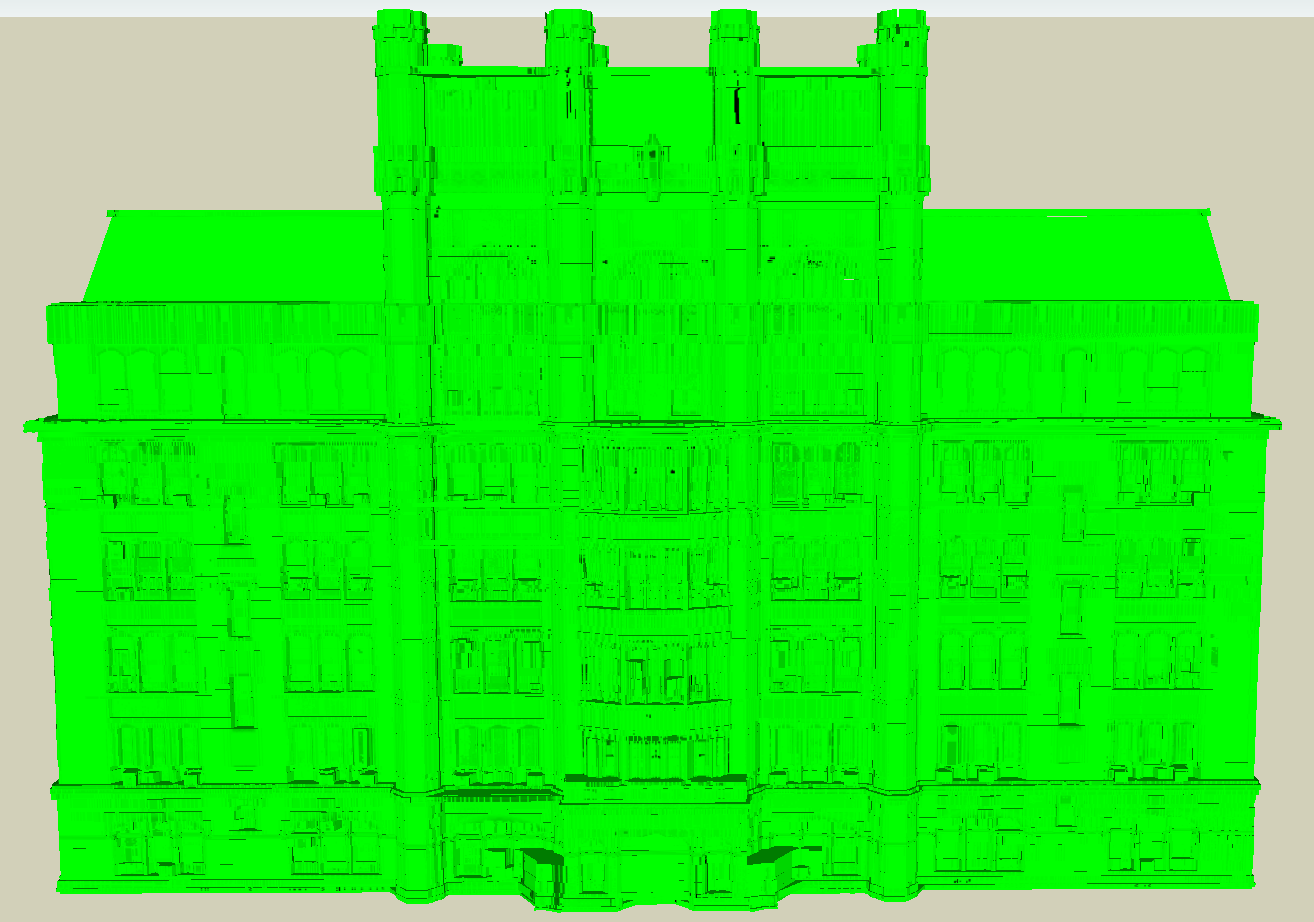
\includegraphics[width=0.2\textwidth]{IR_skp_error_face_1000_4_1_paper.png} \\
(a) & (b)
\end{tabular}
\end{center}
\caption{The deviation mapping of the 3D point cloud. (a) the result with $\tau_r$ = 4 and $\tau_d$ = 32.
(b) the result with $\tau_r$ = 1 and $\tau_d$ = 4. }
\label{fig:EM}
\end{figure}
%%% End of Figure

To visualize the error between real 3D data and the inferred model,
we generated the deviation mapping images which are depicted in \Fig{EM}.
Basically, for each face $p$ of $M$, a corresponding texture image is computed.
The intensity of each pixel in the texture image
is determined by the error of the corresponding 3D points computed by Equation \ref{eq_em}.
The accuracy of the reconstructed model is mainly controlled by the threshold of Hausdorff distance $\tau_d$
and BPA refinement radius $\tau_r$. $\tau_d$ determines the accuracy of the keyslice detection
and $\tau_r$ determines the accuracy of the boundary vectorization.
Table \ref{tbl_em} lists the relationship among the $\tau_d$, errors, number of faces and model size.
The unit for $\tau_d$ is in pixels and for errors is in millimeters.
The size for original 3D building point cloud is more than 700 MB. From the table, one can see that even
for the most accurate model, the size is dramatically reduced compared with the original 3D point cloud data,
which is desired for web-based applications (\Figd{IR_2_DXF}).

%%%%%%%%%%%%%%%%%%%%%%%%%%%%%%%%
%%%%%%   Conclusion and Future Work%%%
%%%%%%%%%%%%%%%%%%%%%%%%%%%%%%%%
\section{Conclusion and Future Work}

In conclusion, we presented a lightweight 3D modeling of urban buildings from range data.
Our work is based on the observation that buildings can be
viewed as the combination of two basic components, the extrusion and the tapering components.
The efficient and economical techniques proposed here are used to infer
the extruded and tapered unit, and then reconstruct the 3D model via vectorization.
The experimental results on both exterior and interior urban building datasets are presented
to validate the proposed approach.

We have successfully inferred the geometry structure of tapering to a line. As a further step, we will study
how to infer the geometry structure of tapering to a point which appears frequently in Gothic architecture,
like churches. A nice characteristic of this structure is that
the sliced image will converge to a point, which is good clue for inference.
Another work is to investigate the modeling of the ``follow-me'' geometry structure, which
is a useful feature included in Google SketchUp.
The ``follow-me'' structure is a more complicated geometry structure which
exists when the underline geometry structure can be reconstructed by
moving a basic geometry unit along a curve trajectory.
We will carry out a tracking computation to obtain the curve trajectory for inference.



\bibliographystyle{acmsiggraph}
\bibliography{siggraph}

\end{document}
